\documentclass[12pt]{article}

\usepackage[brazilian]{babel}
\usepackage[utf8]{inputenc}

% This first part of the file is called the PREAMBLE. It includes
% customizations and command definitions. The preamble is everything
% between \documentclass and \begin{document}.

\usepackage[margin=1in]{geometry}  % set the margins to 1in on all sides
\usepackage{graphicx}              % to include figures
\usepackage{amsmath}               % great math stuff
\usepackage{amsfonts}              % for blackboard bold, etc
\usepackage{amsthm}                % better theorem environments
\usepackage{framed}
\usepackage{epstopdf}
\usepackage{multirow}

% various theorems, numbered by section

\newtheorem{thm}{Theorem}[section]
\newtheorem{lem}[thm]{Lema}
\newtheorem{prop}[thm]{Proposição}
\newtheorem{cor}[thm]{Corolario}
\newtheorem{conj}[thm]{Conjectura}
\newtheorem{defi}[thm]{Definição}

\DeclareMathOperator{\id}{id}

\newcommand{\bd}[1]{\mathbf{#1}}  % for bolding symbols
\newcommand{\RR}{\mathbb{R}}      % for Real numbers
\newcommand{\ZZ}{\mathbb{Z}}      % for Integers
\newcommand{\col}[1]{\left[\begin{matrix} #1 \end{matrix} \right]}
\newcommand{\comb}[2]{\binom{#1^2 + #2^2}{#1+#2}}


\begin{document}

\nocite{*}

\title{Estruturas de Dados para Séries Temporais}

\maketitle

\section{Introdução}

O estudo de séries temporais é motivado por aplicações que surgem 
em diferentes campos do conhecimento tais como medicina, física, metereologia
and finanças, apenas para citar alguns. Para algumas aplicações envolvendo
séries temporais planílias e bancos de dados são suficiente para a análise
desejada. 

Contudo, existem aplicações em que as séries temporais são muito grandes,
como na análise de dados capturados por sensores em milisegundos ou na
análise de quotes or trades no mercado de ações eletrônicas. Para essas
séries, técnicas tradicionais para armazenar os dados podem ser inadequadas
devido ao consumo de tempo/espaço. Esse cenário motiva a pesquisa de estruturas
de dados e algoritmos para lidar com séries temporais grandes\cite{lala}.

O foco da nossa pesquisa é desenvolver estruturas de dados que permitam
a identificação/descoberta de certos tipos de eventos em uma coleção
de séries temporais. Nós estamos interessados em mudanças significativas
na séries que ocorrem em um intervalo pequeno de tempo. Como exemplo,
vamos considerar a seguintes perguntas que são feitas por analistas
de mercado e criadores de estratégias:

\begin{itemize}
\item Ações no mercado financeiro podem ser caracterizadas pelos seus
preços e volume negociados. Dada uma coleção de séries temporais, cada
uma contendo o preço e o volume negociado de uma ação, medidas em segundos,
durante 10 anos, nós queremos responder consultas como: Em quais intervalos
de tempo de $k$ segundos, a maioria das ações tiveram uma variação de pelo
menos \verb|%p| no seu preço e uma mudança de pelo menos \verb|%v| no volume
negociado?

\item Os preços de duas ações com características similares (ex. pertecem
ao mesmo setor da indústria) normalmente apresentam uma forte conexão. Uma
estratégia popular de negociação no mercado financeiro é estimar a razão
entre o preço de duas ações e então apostar que a razão atual irá
retornar para a estimada quando ela varia significamente. Para implementar
essa estratégia consultas como a seguir são importantes: Em quais intervalos
de tempo de tamanho até $\Delta$ T, a razão entre duas ações variou mais que
\verb|%d|?

\end{itemize}


\subsection{Definição do Problema}

Seja $A = (a_1, a_2, \ldots, a_n)$ uma série temporal com $n$ elementos
e seja um índice de tempo um inteiro do conjunto $\{1, \ldots, n\}$. Nós
usamos dois números positivos, $t$ e $d$, para capturar variações na série
A durante um intervalo de tempo. De forma mais precisa, nós dizemos que um
par de índices $(i,j)$ de $A$ é um evento-($t$,$d$) se $0<j - i \le t$ e $a_j - a_i \ge d$.

Nosso objetivo é criar estruturas de dados para pré-processar/indexar séries temporais
de forma a responder as seguintes consultas em tempo sublinear e com pouco tempo/espaço
de pré-processamento:

\begin{itemize}
\item $AllPairs(t, d)$. Esta consulta retorna todos os eventos-($t$,$d$) na série $A$.
\item $Beginning(t, d)$. Esta consulta retorna todos os índices $i$ tais que existe um
índice $j$ tal que $(i,j)$ é um evento-($t$, $d$) na série $A$.
\end{itemize}

Nos concentramos nas consultas acima pois acreditamos que elas são fundamentais
para o estudo de mudanças rápidas em séries temporais, tendo em vista que 
técnicas desenvolvidas para essas consultas podem ser extendidas para outras
consultas semelhantes.

Para facilitar a apresentação dos resultados, nós iremos nos concentrar
em variações positivas ($d > 0$) nas nossas consultas. Contudo, todas as técnicas
desenvolvidas aqui também se aplicam para variações negativas.

A seguinte notação será útil ao longo do trabalho. O valor-$\Delta$ do par $(i, j)$
é dado por $j - i$ e seu desvio por $a_j - a_i$. Nós dizemos que $i$ é o início
do par $(i, j)$ enquanto $j$ e seu fim.

\subsection{Nossa Contribuição}

Para apreciar nossa contribuição é útil primeiro discutir formas
em pontencial para responder as consultas.

Seja $V$ um vetor de números reais, indexado de $1$ até $n$. A Range
Minimum(Maximum) Query (\verb|RMQ|) sobre $V$, com intervalo $[i,j]$, retorna
o índice de $V$ com menor(maior) valor, entre aqueles no intervalo $[i,j]$.
Esse tipo de consulta é bem estudado pela comunidade de geometria computacional
\cite{lala}. De fato, existem estruturas de dados de tamanho $O(n)$ que respondem
consultas \verb|RMQ|s em tempo constante.

Uma observação crucial é que as consultas $AllPairs(t, d)$ e $Beginnings(t,d)$ podem
ser modeladas por como multiplas consultas $RMQ$s (detalhes na próxima seção). Sendo assim,
usando diretamente estruturas de \verb|RMQ|, consegue-se responder ambas consultas
em tempo $O(n + k)$, onde $k$ é o tamanho da resposta. Essa estratégia é ótima para
o problema \textit{offline}, onde o tempo de pré-processamento é levado em consideração
para avaliar o tempo de consulta.

Quando o tempo de pré-processamento não é adicionado a consulta, é possível conseguir
melhores resultados. Por exemplo, para a pesquisa $AllPairs(t,d)$, nós conseguimos
tempo sublinear armazenando todos os pares ${(i,j)| i < j}$, ordenados de forma crescente
pelos seus valor-$\Delta$, em uma estrutura de dados que suporte \verb|RMQ|s. Apesar 
de essa abordagem ser bastante eficiente em termos de tempo de consulta, o espaço
requirido para implementá-la pode ser proibitivo para algumas aplicações reais, pois
temos que armazenar $\Theta(n)$ pares.

A ideia da nossa abordagem é guardar um conjunto de pares especiais de índices
e não todos os pares possíveis. Nós dizemos que um par de índices de tempo $(i,j)$ é
especial em relação a série temporal $A$ se as seguintes condições valem:
$i < j$, $a_i < \min\{a_{i+1}, \ldots, a_j\}$ e $a_j > \max\{a_i, \ldots, a_{j-1}\}$. 
Se um evento-($t$, $d$) é também um par especial, dizemos que é um evento-($t$, $d$) especial.

Seja $S$ o conjunto de pares especiais da série temporal $A$. Nós propomos uma estrutura
de dados de tamanho $O(|S|)$ que responde as consultas $AllPairs(t,d)$ em tempo $O(k)$,
onde $k$ é o tamanho do conjunto solução. Por outro lado, para consultas $Beginnings(t,d)$,
nós propomos uma estrutura de tamanho $O(|S|\log|S|)$ que apresenta tempo de consulta $O(f(\log f + \log t) + k)$,
onde $f$ é a quantidade de índices distintos que são fins de eventos-($t$, $d$) especiais e $k$ 
é a quantidade de inícios que são respostas a consulta.

Um possível ponto negativo da nossa estratégia é que nossa estrutura de dados pode
ter espaço quadrático no pior caso. Isso acontece, por exemplo, se a série temporal
for uma sequência crescente. Contudo, nós argumentamos que isso não é provável de acontecer.
Primeiro, nós provamos que o número esperado de pares especiais para uma permutação aleatória
de $\{1, \ldots, n\}$ é $O(n)$ com alta probabilidade. Esse resultado é interessante pois o número
de pares especiais de uma série temporal com valores distintos é igual ao número de pares 
especiais de permutação de $\{1, \ldots, n\}$ que a série pode ser facilmente mapeada. Além disso,
nós avaliamos o número de pares especiais de $12$ séries temporais que consistem de preços de ações,
medidas a cada minuto, durante um ano, do mercado de ações brasileiro. Para todas as séries, 
o número de pares especiais nunca excedeu $7.5$ vezes do tamanho da série. 

\subsection{Trabalhos Relacionados}
Na última década, uma considerável quantidade de esforços tem sido
feita para desenvolver ténicas de mineração de dados para séries
temporais com discutido em um recente \textit{survey} por Fu\cite{lala}.
Um importante subcampo de pesquisa apontado por esse survey questiona
como identificar informações representativas para ser usada como medida
de similaridade entre duas ou mais séries temporais. A noção de pares
especiais, apresentada aqui, pode ser útil para esse próposito. O livro
de Shasha e Zhu \cite{lala} revisita algumas estruturas de dados para indexar
séries temporais - \textit{data reduction} e \textit{burst detection}, entre outras
aplicações, são discutidas. O trabalho de Shi e Jaja\cite{lala} apresenta um framework
para explorar padrões temporais de um conjunto de objetos. As consultas deles são relacionadas
ao problema de \textit{orthogonal range search} e podem ser usadas para responder questões
interessantes envolvendo séries temporais, porém, tem um contexto consideravelmente diferente
do nosso.
        
O problema de Range Mininum (Maximum) Query (RMQ) consiste em pré-processar um dado
vetor de entrada de forma que a posição do mínimo (máximo) entre dois índices pode
ser obtida de forma eficiente. O primeiro algoritmo de pré-processamento linear e tempo
de consulta constante para o problema RMQ foi descoberto por Harel e Tarjan\cite{lala}. 
O algoritmo, apesar de um grande passo do ponto de vista teórico, era difícil de implementar.
Depois desse artigo, alguns outros foram publicados propondo ideias mais simples, porém ainda
complexas do ponto de vista de implementação. O trabalho de Bender et al. \cite{lala} apresentou
o primeiro algoritmo realmente simples para RMQ. O algoritmo é baseado na conexão entre RMQ e
o problema de  Longest Common Ancestor (LCA), e tem pré-processamento linear e tempo de consulta
constante e é relativamente simples de implementar. O trabalho de Fischer e Heun\cite{} melhora
o algoritmo em Bender at al. reduzindo constantes na memória e tempo.

Finalmente, nosso problema tem alguma semelhança com um problema clássico em geometria computacional -
\textit{fixed radius near neighbors}. Dado um conjunto de $n$ pontos em um espaço Eucliano de $m$ dimensões
e uma distância $d$, o problema consiste em reportar todos os pares de pontos com distância de até $d$.
Bentley et al.\cite{lala} apresentaram uma algoritmo que reporta todos os $k$ pontos que satisfazem
essa propriedade em $O(3^m\times n + k)$. A mesma abordagem pode ser aplicada se um conjunto $\{d_1, d_2, \ldots, d_m\}$ é dado, um para cada dimensão. Contudo, não é claro para nós se ideias similares podem ser aplicadas
para gerar todos os pares com distância \textit{não} menor que $d$ ou, como no caso do nosso problema, não 
maior que $d_1$ na primeira dimensão e não menor que $d_2$ na segunda.


\subsection{Organização da Dissertaçao}
 
\section{Conceitos Básicos}

Nessa seção nós apresentamos observações/resultados que são úteis para tratar
tanto a consulta $AllPairs(t, d)$ quanto para o $Beginnings(t, d)$.

Nossa primeira observação é que é fácil encontrar todos os eventos-($t$,$d$) que possuem
um dado índice $i$ como início. Para isto, nós precisamos de uma estrutura de dados que
suporte consultas RMQ que suporte consultas pelo maior elemento de um intervalo sobre
um vetor $A$ em tempo constante e que tenha tempo/espaço de pré-processamento linear,
como discutido na seção de trabalhos relacionados. Com uma estrutura dessas, nós podemos
chamar o procedimento \verb|GenEventStart|, apresentado na Figura~\ref{lala}, com parâmetros
$(i, i + 1, i + t)$. Esse procedimento quando executado com os parâmetro $(i, low, high)$ gera
todos os eventos-(t,d) com início $i$ e final no intervalo $[low, high]$. Primeiro o procedimento
usa a estrutura de RMQ para achar o índice dentro do intervalo $[low, high]$ de maior valor no 
vetor $A$. Se o desvio ($a_j - a_i$) é menor que $d$ então a busca termina, pois claramente não
há evento-(t,d) que satisfaza a consulta dentro do intervalo. Caso contrário, o procedimento reporta
o par $(i, j)$ e explora recursivamente os intervalos $[low, j - 1]$ e $[j + 1, high]$. Nós sumarizamos
o dito no procedimento~\ref{lala}.

\begin{prop}
Seja $k_i$ a quantidade de eventos-($t$,$d$) que têm início $i$ e fim no intervalo $[low, high]$.
Então, o procedimento \verb|GenEventsStart|$(i, low, high)$ gera todos esses eventos em tempo $O(k_i + 1)$.
\end{prop}
\begin{proof}
lala
\end{proof}


\begin{figure}
\fbox {

\begin{minipage}{12 cm}

{\tt GenEventsStart}($i$,$low$,$high$)
  
\hspace{1cm}  {\bf If} $high \geq low$
  
\hspace{2cm}  $j \leftarrow RMQ(low,high)$
  
\hspace{2cm}  {\bf If} $a_j -a_i \geq d$  \,\, (*)
    
\hspace{3cm}     Adiciona o par $(i,j)$ à lista de eventos-$(t,d)$  \,\, (**)
     
\hspace{3cm}     {\tt GenEventsStart}($i$,$low$,$j$-1)
     
\hspace{3cm}     {\tt GenEventsStart}($i$, $j$+1,$high$)
   
\hspace{2cm}  {\bf End If  } 

\hspace{1cm} {\bf   End If }

\end{minipage}

}
\end{figure}


Nós vamos considerar também um procedimento análogo, chamado \verb|GenEventsEnd|, que recebe
como entrada uma tupla $(j, low, high)$ e gera todos os eventos-$(t,d)$ que tem $j$ como final
e o ínicio no intervalo $[low, high]$. 

O seguinte Lema~\ref{lala} motiva nosso foco em pares especias para responder as consultas
$AllPairs(t,d)$ e $Beginnings(t,d)$.

\begin{lem}  
Seja $(i, j)$ um evento-$(t,d)$. Então, as seguintes condições valem:
\begin{enumerate}
\item Existe um índice $i*$ tal que $(i*, j)$ é um evento-$(t,d)$ e $i*$ é o ínicio de um 
evento-$(t,d)$ especial. 
\item Existe um índce $j*$ tal que $(i, j*)$ é um evento-$(t,d)$ e $j*$ é o final de um
evento-$(t,d)$ especial.
\end{enumerate}
\end{lem}
\begin{proof}
Nos iremos apenas prova (i), já que a prova para o segundo é análaga. Seja $i*$ o índice
de tempo do elemento de $A$ com menor $a_i*$ entre os índices no intervalo $\{i, \ldots, j -1\}$.
Em caso de empates, considere o maior índice. Como $a_i* \le a_i$, $i \le i* < j$ e $(i, j)$ é um
evento-$(t,d)$, temos que $(i*, j*)$ é também um evento-$(t,d)$. Seja $k*$ o índice do elemento
de $A$ com maior valor entre aqueles no conjunto $\{i* + 1, \ldots, j\}$. O par $(i*, k*)$ é 
tanto um par especial quanto um evento-$(t,d)$, que conclui a demonstração.
\end{proof}

Nosso último mostra que o conjunto de pares especiais para uma dada série de tamanho
$n$ pode ser gerado em tempo $O(n + |S|)$. 

\begin{prop}
Seja $S$ o conjunto de pares especiais para uma série $A$ de tamanho $n$. Então, 
$S$ pode ser construido em tempo $O(|S| + n)$.
\end{prop}
\begin{proof}
A corretude é trival. O tempo de execução do procedimento é proporcional ao
número de chamdas recurvas que ele executa. O fluxo de execução pode ser visto
como uma árvore binária onde cada nó corresponde a uma chamada recursiva.
Note que em todos nós internos um novo evento-$(t,d)$ é encontrado. E como
em toda árvore binária o número de nós é no máximo duas vezes o número de nós
internos, o número de chamadas recursivas é no máximo $2k_i$.
\end{proof}

\section{Estruturas de Dados para Detecção de Variações Rápidas em Séries Temporais - AllPairs}

\subsection{Lista Ordenada}

O pré-processamento consiste em montar $n$ listas ordenadas $L_1, L_2, \ldots, L_n$, 
essas listas mantém pares da série inicial. Para cada par ordenado da série de entrada $(a_i, a_j)$, com $i < j$ e $a_i < a_j$,
armazenamos a tupla $(a_j - a_i, i, j)$ na lista de índice $j - i$.
Após todos os pares serem inseridos as listas são ordenadas de forma decrescente. A Figura~\ref{fig:exemplolista} apresenta um exemplo.
Desta forma, para responder uma consulta $(t, d)$ simplesmente achá-se as soluções
dentro de cada lista $L_1, L_2, \ldots, L_t$. Fixada uma lista $L_i$ é simples
encontrar as soluções dentro dela, uma vez que os pares armazenados na mesma
estão ordenados de forma decrescente, basta começar a iterar do início
da lista e continuar enquanto os elementos tiverem valor maior ou igual a	$d$.
O pseudo-código na Figura~\ref{fig:listaquery} mostra o algoritmo. Uma observação importante é 
que o custo para achar as soluções dentro da lista $L_i$ é no máximo $k_{s_i} + 1$,
 onde $k_{s_i}$ é a quantidade de tuplas que correspondem a soluções dentro da $L_i$. 

% inserir figura
\begin{center}
\begin{figure}
\begin{framed}
Série de Entrada: $<3, 2, 5, 8>$ \\
$L_1: (3, 2, 3), (3, 3, 4)$ \\
$L_2: (6, 2, 4)$ \\
\end{framed}
\label{fig:exemplolista}
\caption{Índices começam por $1$}
\end{figure}
\end{center}


\begin{center}
\begin{figure}
\begin{framed}

{\bf ListaOrdenadaQuery}$(t, d)$

\hspace{1cm} {\bf For} $i \in [1, t]$

\hspace{2cm} $m \leftarrow 0$

\hspace{2cm} {\bf While} $m < |L_i|$ and $L_i[m][0] \ge d$

\hspace{3cm} Reporte o par $(L_i[m][1], L_i[m][2])$

\hspace{3cm} $m \leftarrow m + 1$
\end{framed}
\label{fig:listaquery}
\caption{Consulta}
\end{figure}
\end{center}

Com o mencionado, essa estratégia tem tempo de pré-processamento $O(n^2 \log n)$(ordenar uma lista de $n^2$ elementos) 
e tempo de pesquisa de no máximo $\sum_{i = 1}^{t} k_{s_i} + 1$, ou seja, $O(k + t)$,
onde $k$ é a quantidade de respostas a consulta $(t,d)$ feita.

\subsection{Multiplas RMQ}

Como apresentado na seção \ref{lala}, o RMQ é o problema de 
encontrar o mínimo (máximo) de um intervalo de vetor de forma 
eficiente. Como foi mostrado existem poderosas estruturas
de dados que permitem responder consultas RMQ em tempo $O(1)$, a partir de um pré-processamento $O(n)$. 
Nessa seção será apresentado um algoritmo que a partir de uma estrutura de RMQ para série
de entrada responde consultas $(t, d)$ em $O(n + k)$. 

A ideia principal do algoritmo é fixar um $i$ e encontrar todos os pares $(i, j)$ 
que são solução da pesquisa, ou seja, os pares em que $a_i$ é o menor elemento. 
Suponha que $a_m$ é o maior elemento dentro do intervalo $[i+1, i+2, \ldots, i+t]$, 
note que se $(i, m)$ não for uma solução para pesquisa $(t, d)$ (isto é, $a_m - a_i < d$) então
nenhum outro elemento do intervalo formará um par com $a_i$, por outro lado, se $a_m$  
forma solução com $a_i$, podemos reportar o par $(i, m)$ e seguir recursivamente explorando os intervalos
$[i+1, \ldots, m - 1]$ e $[m + 1, \ldots, t]$. Repare que, como a série foi
pré-processada e existe uma estrutura de RMQ para a mesma, o elemento $a_m$
pode ser encontrado em $O(1)$.

Achar soluções a partir de um elemento fixo é fundamental para a sequência
desse trabalho, sendo assim, o pseudo-código dessa etapa está em uma função separada chamada \verb|FindByFirst|,
apresentada na Figura~\ref{findbyfirst}. Repare que o pseudo-código assume que há acesso global a série
de entrada $A$ e que existe uma estrutura de RMQ para a mesma ($rmqA$). Com as mesmas
ideias aplicadas no \verb|FindByFirst|, podemos criar uma outra versão, o \verb|FindBySecond|, que
acha todas as soluções quando o maior elemento do par está fixado. O \verb|FindBySecond| está apresentado
nessa seção por completude, ele só será utilizado em uma seção posterior.

Finalmente, para de fato responder uma consulta, todas as soluções podem ser encontradas variando-se o 
elemento fixado da série e usando o \verb|FindByFirst| para encontrar as soluções com
o primeiro elemento fixado. A Figura~\ref{queryrmq} contém  o pseudo-código completo.

\begin{figure}
\begin{framed}
{\bf QueryRMQ}(t, d)

\hspace{1cm} {\bf For} $i \in [1, n]$:

\hspace{2cm} {\bf FindByFirst}(i, i, i + t, t, d):
\end{framed}
\label{queryrmq}
\caption{Responde a uma consulta $(t,d)$ a partir de uma estrutura de RMQ.}
\end{figure}


\subsection{Abordagem baseada em Pares Especiais}
Seja $S$ o conjunto de pares especiais de uma série temporal $A = (a_1, \ldots, a_n)$. 
Nossa solução armazena $S$, ordenado de forma crescente pelos valores $\Delta$, em 
um vetor $V$; empates são decididos arbitrariamente. Além disso, nossa estrutura utiliza
uma RMQ ${\cal D}$ de tamanho $O(|S|)$ para responder a seguinte consulta: dado dois valores
$t^*$ e $d^*$, reporte o subconjunto de pares especiais de $S$ com valor-$\Delta$ de até $t^*$ e 
desvio de ao menos $d*$. Finalmente, nos usamos outras duas RMQ auxiliares ${\cal D}_{min}$ e 
${\cal D}_{max}$ de tamanho $O(n)$ para podermos charmar, respectivamente, os procedimentos \verb|GenEventsEnd|
e \verb|GenEventStart| sobre $A$. 

Para responder a consulta $AllPairs(t, d)$ nos executamos duas fases. Na primeira, 
nos encontramos todos os eventos-$(t,d)$ especiais de $V$ usando a RMQ ${\cal D}$.
Então, na segunda fase, nos usamos esses eventos-$(t,d)$ especiais e as estruturas 
${\cal D}_{min}$ e ${\cal D}_{max}$ para encontrar os outros eventos-$(t,d)$. As duas fases
são apresentadas em detalhes abaixo.

\textbf{Fase 1}. Seja $k^*$ o índice do último par em $V$ entre aqueles com valor-$\Delta$
de até $t$. Nós usamos ${\cal D}$ para executar consultas de máximos em intervalos para
encontrar os eventos-$(t,d)$ em $V[1, \ldots, k^*]$. De forma mais precisa, seja $i$ o índice
de $V$ o índice de $V$ retornado por uma consulta de máximo em $V$ entre os elementos de
índice $[1, k^*]$. Se o desvio do par armazenado em $V[i]$ é menor que $d$ nós podemos
terminar a busca, já que nenhum outro par em $V[1, \ldots, k^*]$ terá desvio de ao menos $d$.
Caso contrário, adicionamos o par $V[i]$ a lista ${\cal L}$ e proseguimos recursivamente 
nos subvetores $V[1, \ldots, i - 1]$ e $V[i + 1, \ldots, k^*]$. No final a lista ${\cal L}$ terá
todos os eventos-$(t,d)$ especiais. 

\textbf{Fase 2}. Esta fase pode ser dividida em duas etapas.

\textbf{Fase 2.1}. Nessa subfase, geramos o conjunto de início distintos de eventos-$(t,d)$ especiais.
Primeiro, nós geramos a lista ${\cal E}_L$ de fins em ${\cal L}$, que
pode ser feito em $O(|L|)$ mantendo um vetor de $0-1$ para evitar repetições de fins. Então,
chamamos o procedimento \verb|GenEventsEnd(j, j - t, j - 1)| para todo $j \in {\cal E}_L$. É 
importante lembrar que \verb|GenEventsEnd| utiliza a estrutura ${\cal D}_{min}$. Durante o processamento
do \verb|GenEventsEnd| nos armazenamos todos os inícios de eventos-$(t,d)$ encontrados em uma lista
${\cal B}$. Novamente, utilizamos um vetor $0-1$ para evitar repetições entre inícios.

\textbf{Fase 2.2} Nessa subfase, geramos todos os eventos-$(t,d)$ que têm inícios armazenados
na lista ${\cal B}$. Para isto, chamamos o procedimento \verb|GenEventsStart(i, i + 1, i + t)| para
todo $i \in B$. Novamente, é importante lembrar que o esse procedimento utiliza a estrutura ${\cal D}_{max}$.
Finalmente, a lista de pares retornada pelo procedimento \verb|GenEventsStart| apresenta todos, e somente
estes, eventos-$(t,d)$ que estamos procurando.

A discussão dessa seção é sumarizada pelo teorema abaixo.

\begin{thm}
O procedimento acima gera todas as $k$ soluções para uma consulta $AllPairs(t, d)$ em tempo $O(k + 1)$
e com $O(|S| + n)$ de espaço e tempo de pré-processamento.
\end{thm}
\begin{proof}
No final da Fase 1, nós temos todos os eventos-$(t,d)$ especias,
isto é feito em tempo $O(k)$. No começo da Fase 2.1,
obtemos o conjunto $E_{\cal{L}}$ contendo os fins distintos,
novamente em tempo $O(k)$. Pelo item (ii) do Lema~\ref{lem:SpecialPairsProperty}
o conjunto $B$ contendo todos os inícios de eventos-$(t,d)$ pode ser gerado a partir
dos fins em $E_{\cal{L}}$. Nós obtemos o conjunto $B$ em tempo $O(K)$ chamando o {\tt GenEventsEnd}$(j,j-t,j-1)$
para cada $j \in E_{\cal{L}}$. Finalmente, gastamos mais $O(k)$ para gerar todos os eventos-$(t,d)$
chamando {\tt GenEventsStart}$(i,i+1,i+t)$ para cada $i \in B$.
\end{proof}


\section{Gerando Pares Especiais}

O conjunto $S$ de pares especiais de uma série temporal $A$, de tamanho $n$, pode ser obtido
em tempo $O(n + |S|)$ chamando o pseudo-código apresentado na Figura~\ref{fig:GenSpecialPairs}
com parâmetros $(1, n)$. Primeiro, o procedimento usa uma estrutura de RMQ para calcular
em tempo constante o índice $i$ de menor valor no intervalo $[low, high]$ e outra
para calcular o índice $j$ de maior valor no intervalo $[i + 1, high]$. 
O loop {\bf While} encontra todos os pares especiais que tem como início o índice $i$.
Finalmente, o procemindo explora recursivamente os intervalos $[low, i - 1]$ e $[i + 1, high]$.

Para entender a corretude do procedimento basta notar que se $i$ for o índice
do menor elemento do intervalo $[low, high]$ então, pela difinição de pares especiais,
é impossível existir um par especial $(x, y)$ tal que $low \le x < i$ e $i < y \le high$.

Por fim, note que a loop {\bf While} só itera no máximo uma vez mais que a quantidade
de pares speciais com início $i$ e a cada chamada recusiva reduzimos o tamanho do intervalo
$[low, high]$ em pelo menos $1$. Sendo assim, o tempo de execução é $O(n + |S|)$.


\begin{figure}

\fbox {

\begin{minipage}{12 cm}

\small


{\tt GenSpecialPairs}($low$,$high$)
  
\hspace{1cm}  {\bf If} $high \geq low$
  
\hspace{2cm}  $i \leftarrow RMinQ(low,high)$

\hspace{2cm}  $j \leftarrow RMaxQ(i + 1, high)$
  
\hspace{2cm} {\bf While} $i < j$ and $a_j - a_i \ge d$

\hspace{3cm}  Adicine o par $(i, j)$ à lista de pares especiais

\hspace{3cm}  $j \leftarrow RMaxQ(i, j - 1)$
  
\hspace{2cm} {\tt GenSpecialPairs}$(low,i-1)$
     
\hspace{2cm}  {\tt GenSpecialPairs}$(i+1,high)$
     
\hspace{1cm} {\bf   End If }

\end{minipage}

}

\caption{Procedure to generate all special pairs}
\label{fig:GenSpecialPairs}
\end{figure}


\section{Beginnings}

\subsection{Estrutura baseada em Pares Especiais}

Para explicar nossa estrutura precisamos introduzir novas notações.
Para um intervalo $[i, j]$, definimos $S_{[i,j]}$ como o conjunto
de pares especiais cujos valores-$\Delta$ estão dentro do intervalo $[i, j]$.
Seja $L_{[i, j]}$ a lista obtida como segue: primeiro ordenamos os pares
em $S_{[i, j]}$ em ordem decrescente de seus desvios. Depois, passamos na lista
e removemos os pares especiais sempre que seu final já apareceu como final de outro
par especial na lista.

Para responder a consulta $Beginnings(t,d)$ precisamos de uma árvore binária ordenada ${\cal T}$
onde cada nó é associado a um subintervalo de $[1, n - 1]$. Mais precisamente, a raiz de ${\cal T}$
é associada ao intervalo $[1, n - 1]$. Se um nó $v$ é associado com o intervalo $[i, \ldots, j]$ então
seu filho à esquerda é associado ao intervalo $[i, \lceil \frac{(i + j)}{2} \rceil]$ e seu filho à direita associado
a $[\lceil \frac{(i + j)}{2} \rceil  + 1, j]$. Além disso, cada nó de ${\cal T}$ aponta para a lista associada a seu intervalo, isto é, o nó $v$ associado com o intervalo $[i, j]$ aponta para a lista $L_{[i, j]}$. A Figura\ref{alla}
mostra um exemplo para séries temporais com $n = 8$ elementos. O tamanho da estrutura é $O(\min\{n^2, |S|\log n\})$ porque cada par especial pode aparecer em até $\log n$ listas $L_{[i, j]}$ e o tamanho de cada lista
é no máximo $n$, uma vez que cada fim aparece no máximo uma vez.

Para responder a consulta $Beginnings(t,d)$ o procedimento executa duas fases. Na primeira, 
ele obtém todos os fins de eventos-$(t,d)$ especiais. Na segunda fase, usa os fins para obter
os inícios dos eventos-$(t,d)$.

A corretude desse procedimento é baseada no item $(ii)$ do Lema~\ref{ala} porque se $i$ é um
início de um evento-$(t,d)$ então existe um fim $j*$ de um evento-$(t,d)$ especial tal que $(i, j*)$
é um evento-$(t,d)$. E, como será visto, o fim $j*$ é achado na Fase1 e usado para achar $i$ na Fase2.

\textbf{Fase 1}. Primeiramente, achamos o conjunto $S$ de nós em ${\cal T}$ cujos intervalos associados
formam uma partição do intervalo $[1, t]$. No exemplo da Figura 2, para $t = 6$, $S$ consiste de 
dois nós: um associado ao intervalo $[1, 4]$ e outro com o intervalo $[5, 6]$. Pode ser mostrado 
que é sempre possível achar em tempo $O(\log n)$ um conjunto $S$ com até $\log t$ nós. Uma forma
de ver isto é perceber que ${\cal T}$ é exatamente a primeira camada de uma \textit{Range Search Tree 2D}
(\cite{alla}).

\begin{figure}[htp]
\begin{center}
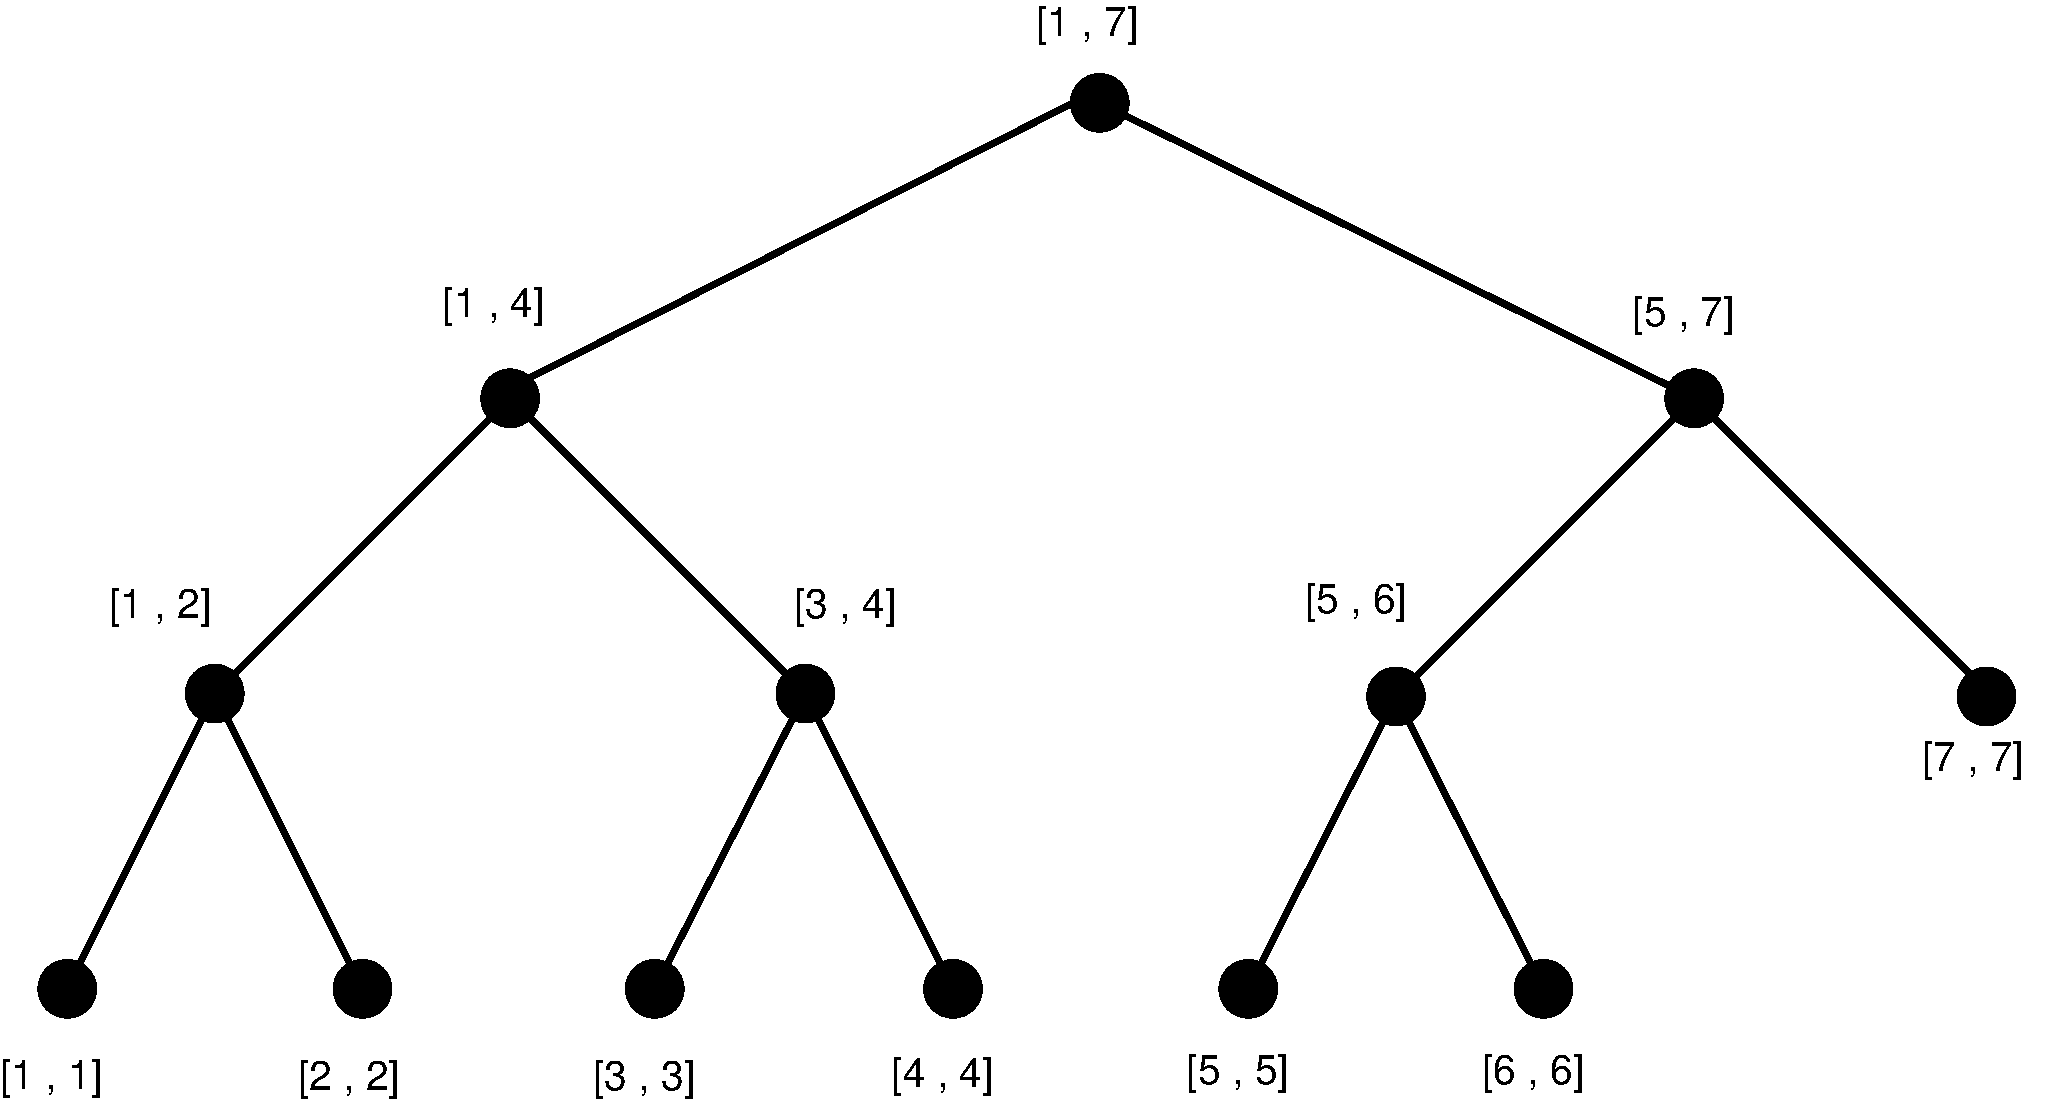
\includegraphics[scale=0.2]{arvore.pdf}
\caption{Uma árvore binária ordenada para $n = 8$. A raiz de ${\cal T}$ possui um pointeiro para a lista $L_{[1,7]}$ enquanto seus filhos à esquerda 
e a direita, respectivamente, têm ponteiros para $L_{[1,4]}$ e $L_{[5,7]}$. }
\label{fig:binary_tree}
\end{center}
\end{figure}



Então, para cada nó $v \in S$,  procedemos como segue: percorremos a lista de pares especiais associada
com $v$; se o par especial atual tem desvio maior ou igual a $d$, nós verificamos se seu final já foi a adicionado a lista de finais $E_f$. Se não foi, nós adicionamos o final a $E_f$; caso contrário, nós seguimos
em frente. O percorrimento é interompido quando encontramos um par especial com desvio menor que $d$
ou chegamos ao final da lista. Esse passo custa no máximo $O(|E_f| \log t)$ porque cada final aparece no máximo
em $\log t$ listas.

\textbf{Fase 2}. A segunda fase pode ser divida em três fases menores:

\textbf{Fase 2.1}. Nessa subfase, ordenamos os fins em $E_f$ em tempo $O(\min\{n, |E_f|\log|E_f|\})$  
usando ou um \textbf{bucket sort} ou um \textbf{heapsort} dependendo se $|E_f|$ é maior que $n/\log n$ ou
não. Seja $e_1 < e_2 < \ldots < e_f$ os fins em $E_f$ ordenados.

\textbf{Fase 2.2}. Primeiro, defina, para um fim $e_j \in E_f$, a função $clp(e_j) = e_{i*}$,
onde $i = \max\{i|e_i \in E_f \text{e} e_i < e_j \text{e} a_{e_i} \ge a_{e_j}\}$. De outra forma,
$clp(e_j)$ retorna o fim a esquerda de $e_j$, que tem índice menor que $e_i$ e valor maior ou 
igual a $a_{e_j}$. Para garantir que todo $clp(e_j)$, para $j = 1, \ldots, |E_f|$, é válido nós
assumimos que $E_f$ contém um elemento artificial $e_0$ tal que $e_0 = 0$ e $a_{e_0} = \inf$.
Por exemplo, seja $E_5 = \{e_1, e_2, e_3, e_4, e_5\}$ uma lista ordenada de fins, onde 
$(e_1, e_2, e_3, e_4, e_5) = (2,3,5,8, 11)$ e $(a_{e_1}, a_{e_2}, a_{e_3}, a_{e_4}, a_{e_5}) = (8,5,7,6,4)$.
Nós temos que $clp(e_4) = e_3$ e $clp(e_3) = e_1$. Os $clp$'s podem ser calculados em $O(|E_f|)$ como
descrito mais abaixo. 

\textbf{Fase 2.3}. Para gerar os inícios de eventos-$(t,d)$ a partir dos fins em $E_f$, o procedimento
na Figura~\ref{lala} é executado. O procedimento itera sobre todos os fins em $E_f$ e guarda na variável
$CurrentHigh$ o menor índice $j$ para qual todos os inícios maiores que $j$ já foram gerados. 
Essa varíavel é inicializada com o valor $e_f - 1$ pois não há início maior que $e_f - 1$. Para
cada fim $e$ o procedimento procura por inícios no intervalo $[max\{e_i - t, clp(e_i)\}, CurrentHigh]$.
Note que ele não procura inícios no intervalo $[e_i - t, clp(e_i)]$ uma vez que todo início nesse
intervalo que pode ser gerado por $e_i$ pode também ser gerado por $clp(e_i)$ (porém o contrário
não é verdade). De fato, esta é a razão para termos calculado os $clp$'s - eles evitam que um 
início seja gerado mais de uma vez. Seguindo, a varíavel $CurrentHigh$ é atualizada e uma nova
iteração começa. Essa subfase pode ser implementada em tempo $O(|E_f| + k)$, onde $k$ é a quantidade
de inícios geradas. 

A discussão pode ser resumida no seguinte teorema.

\begin{thm}
Existe uma estrutura de dados de tamanho $O(|S|\log |S|)$ que suporta a pesquisa $Beginnings(t,d)$
em termpo $O(\log n + f.(\log f + \log t) + k)$, onde $k$ é o tamanho do conjunto solução e $f$ 
é o número de fins distintos de eventos-$(t, d)$ especiais. 
\end{thm}


\begin{figure}

\fbox{

        \begin{minipage}{13 cm}

        \small

        CurrentHigh $\leftarrow e_f -1$

        {\bf  For} $i=f $ downto 1.

        \hspace{1cm} {\tt GenEventsEnd } $(e_i, \max \{e_i -t, clp(e_i)\}, CurrentHigh)$

        \hspace{1cm}  CurrentHigh  $\leftarrow  \max \{ e_i -t,  clp(e_i) \} $

        {\bf End For}

        \end{minipage}

}

\caption{Procedure to generate the beginnings}
\label{fig:beginnings} 
\normalsize

\end{figure}

É importante ressaltar que, com algum esforço, é possível reduzir o fator 
$\log f$ na complexidade acima. A ideia principal é criar uma estrutura de RMQ
para cada lista $L_{i,j}$ e ordenar pares especiais em  $L_{i, j}$ pelo seus fins
e não por seu desvio. Desta forma, conseguimos trocar a ordenação na fase 2.1 
uma operação mais rápida de merge. EXPLICAR EM DETALHES.


\subsubsection{Calculando os $clp$s}
A Figura~\ref{fig:clp} mostra o pseudo-código do procedimento
para calcular $clp$'s em tempo $O(|E_f|)$. O loop externo
claramente é executado $O(|E_f|)$ vezes. Além disso, 
cada fim é adicionado a $Q$ no máximo uma vez e a cada iteração
do {\bf While} um fim é removido de $Q$. Sendo assim,
o loop {\bf While} também leva tempo linear.


\begin{figure}

\fbox{

        \begin{minipage}{13 cm}

        \small

        $Q \leftarrow \emptyset $; Add $e_f$ to the tail of queue $Q$.

        {\bf  For} $i=f-1 $ downto 0.

        \hspace{1cm} $e \leftarrow Q.tail$

        \hspace{1cm} {\bf While} $a_e  < a_{ e_i} $

        \hspace{2cm} Remove $e$ from $Q$

        \hspace{2cm} $clp(e) \leftarrow e_i$ 

        \hspace{2cm} $e \leftarrow Q.tail$ 

        \hspace{1cm} {\bf End While}

        \hspace{1cm} Add $e_i$ to the tail of $Q$.

        {\bf End For}

        \end{minipage}

} % close fbox

\caption{Procedure to generate the clp's}

\label{fig:clp} 

\normalsize

 \end{figure}
 %\end{minipage}


\section{Quantidade Pares Especiais}

Como o tempo e espaço de pré-processamento da nossa estrutura de dados
depende do número de pares especiais, essa seção discute alguns resultados
teóricos e prático relacionados a esse número.

Claramente, o número de pares especiais de uma série temporal é pelo 
menos 0 e no máximo $n(n - 1)/2$, onde o limite inferior(superior) é
atingido para uma sequência decrescente(crescente). A seguinte proposição
mostra que o valor esperado do número de pares especiais para uma permutação
aleatória do $n$ primeiros elementos é $n - H_n$. Esse resultado é interessante
do ponto de vista que a quantidade de pares especiais em uma série temporal 
é igual ao de uma permutação que esta série pode ser mapeada, como mostrado abaixo.

\begin{prop}
Seja $S$ o conjunto de pares especiais de uma série 
temporal escolhida de forma uniforme randomicamente de um conjunto de $n$ elementos.
Então, o valor esperado de $S$ é $n - H_n$, onde $H_n$ é o n-ésimo termo 
da série harmônica.
\end{prop}
\begin{proof}
Seja $E[X]$ tamaho esperado da lista $S$ de pares especiais.
Além disso, seja $X_{i,j}$ uma variável aleatória indicadora que
tem valor $1$ se o par de índices $(i,j)$ pertecem a $S$ e $0$, caso contrário.

Pelas definições anteriores, 
$$E[X] = E[\sum\limits_{i=1}^{n-1} \sum\limits_{j=i+1}^{n}X_{i,j}].$$

Pela linearidade do valor esperado, temos que:

$$E[\sum\limits_{i=1}^{n-1} \sum\limits_{j=i+1}^{n}X_{i,j}] = \sum\limits_{i=1}^{n-1} \sum\limits_{j=i+1}^{n} E[X_{i,j}].$$

Desde que $E[X_{i,j}] = \frac{1}{(j-i+1)(j-i)} = \frac{1}{j-i} - \frac{1}{j-i+1}$, temos:

$$E[X] = \sum\limits_{i=1}^{n-1} \sum\limits_{j=i+1}^{n}
\left (\frac{1}{j-i} - \frac{1}{j-i+1} \right )
= \sum\limits_{i=1}^{n-1} \left (1 - \frac{1}{n-i+1} \right)
= n - \sum\limits_{i=1}^{n} \frac{1}{i}  =  n - H_n.$$
\end{proof}

A seguinte proposição, cuja a prova deixamos para o apêndice, mostra que 
a cardinalidade de $S$ é altamente concentrada no seu valor médio.

\begin{prop}
Seja $c>0$ um número real, então $Pr\{X \ge c.n\} \le \frac{c' \log n}{c^2n}$, onde
$c'$ é uma constante positiva fixada.
\end{prop}

Como nossa pesquisa é fortemente motivada por aplições que surgem no mercado
financeiro, nós também avaliamos o número de pares especiais para séries temporais
contendo os preços de seis diferentes ações do mercado Brasileiro de ações, observadas
de minuto a minuto, durante um período de um ano. 

Nós observamos que a razão entre o número de pares especiais e o tamanho da série fica no intervalo
$[3.37, 7.23]$, com valor médio $5.08$. Estes resultados sugerem que as estruturas propostas aqui são
 efetivas em termos de consumo de espaço para aplicações reais.  


\subsection{Extensões para outras consultas}
 Explicar nossa abordagem e outras triviais

\section{Avaliação Experimental}

Nessa seção buscamos avaliar as estruturas propostas sobre o enfoque experimental.



\subsection{Corpus}

Nosso corpus é formado de doze séries, as 6 primeiras são séries advindas do mercado financeiro, 
cada série apresenta os preços de minuto à minuto de uma dada ação durante o período de um ano. 
As outras seis são simplismente as 6 primeiras séries invertidas e são usadas para modelar
o comportamento de pesquisas com desvios negativos. Por exemplo, uma consulta $AllPairs(2, -3)$
em uma série $A=(4, 1, 5, 2)$ é equivalente a uma pesquisa $AllPairs(2, 3)$ na série $A=(2, 5, 1, 4)$,
o mesmo vale para consulta $Beginnings$.

A Tabela~\ref{4} mostra o tamanho e quantidade de pares especiais para cada uma dessas séries.
Os números entre parênteses são a razão entre o número de pares especiais e o tamanho das séries.
A tabela também apresenta a quantidade de pares especiais para as séries invertidas.
 
\begin{table}
\small
\begin{center}
\begin{tabular}{|c|c|c|c|}
\hline
 {\bf Série Temporal}  & {\bf Tamanho} ($n$) & {\bf $\#$ pares especiais} & {\bf $\# $ pares especiais na série invertida} \\ 
\hline
 1 & 191.672   & 1.386.964 ( 7.23 ) &  850.356 (4.44) \\
\hline
 2 & 195.708 & 1.305.974  (6.67) & 928.878 (4.75)\\
\hline
 3 & 142.941 &   713.019 (4.98) & 482.417  (3.37) \\
\hline
 4 & 137.257 &  968.666  (7.06) &  548.780 (4)\\
\hline
 5 & 179.443 & 853.435 (4.76) &  812.149 (4.53) \\
\hline
6  &  177.631 &  910.915 (5.13) &  720.781  (4.06) \\ \hline
\end{tabular}
\end{center}
\label{tab:Special-pairs}
\caption{A quantidade de pares especiais para algumas séries reais}
\normalsize
\end{table}


\subsection{Ambiente}

A implementação de todas as heurísticas foi feita em \verb|C++|, o compilador
utilizado foi \verb|o g++ 4.4.3|, com flag de otimização \verb|-O2|. O computador
utilizado para os testes tem \verb|3GB| de RAM e processador Intel(R) Core(TM)2 Duo CPU, T6600  @ 2.20GHz
de 64 bits. O sistema operacional utilizado foi o Ubuntu 10.04 LTS - Lucid Lynx.


\subsection{RMQs}

De acordo com o artigo~\ref{lala}, a implementação mais eficiente, dentre aquelas
de pré-processamento linear,  para séries de tamanho até $10^6$ é {\tt RMQBucket}.
Com isso em vista, utilizamos duas essa implementação de {\tt RMQ} e também a estrutura
{\tt RMQSt} descrita. Nessa seção apresentamos experimentos medindo o tempo de pré-processamento
e consulta de ambas implementações.


\subsection{AllPairs}

\subsubsection{Pré-processamento}
Nessa seção reportamos os experimentos realizados para a consulta $AllPairs(t,d)$.
Nós comparamos nossa estrutura baseada em Pares Especiais com a estratégia simples onde para cada possível
início utiliza-se o procedimento {\tt GenEventsStart} para encontrar os eventos-$(t,d)$ com o dado início,
chamaremos essa estratégia de {\tt SimpleRMQ}.

Um ponto importante na comparação entre as duas estruturas é a implementação de RMQ usada pela estratégia. 
Entre as duas implementações principais, {\tt RMQBucket} e {\tt RMQSt}, partições se mostrou a única víavel para 
nossa estratégia baseada em pares especiais, devido ao alto consumo de memória da implementação {\tt RMQSt}.
Já para a {\tt SimpleRMQ} apresentamos resultados com as duas implementações.

Na primeira tabela mostramos os tempos de pré-processamento de cada estrutura, os tempos são a média 30 execuções.
Nossa estrutura apresenta o maior tempo de pré-processamento,  sendo de 1.3 a 2 vezes mais lenta que a {\tt SimplesRMQ}
 com {\tt RMQBucket} e entre $9$ e $20$ vezes mais lenta que a {\tt SimplesRMQ}  com {\tt RMQSt}.

\begin{verbatim}
SerieID, SerieSize, Fpairs, RMQBased with RMQBucket, RMQBased with RMQSt, F-pairs with RMQBucket
1, 191672, 1382715, 41.563, 415.833, 814.812
2, 195708, 1304713, 57.493, 468.861, 663.924
3, 142941, 707947, 28.518, 268.233, 381.961
4, 137257, 968732, 26.582, 236.204, 479.918
5, 179443, 846592, 36.51, 324.864, 443.041
6, 177631, 906852, 34.241, 298.42, 452.992
7, 191672, 842686, 38.376, 330.254, 433.988
8, 195708, 925384, 38.556, 336.465, 469.763
9, 142941, 473063, 28.937, 249.367, 274.604
10, 137257, 545799, 26.987, 230.639, 275.893
11, 179443, 792811, 36.868, 317.634, 429.943
12, 177631, 710068, 34.704, 303.836, 370.179
\end{verbatim}


Apesar do maior tempo de pré-processamento, como será mostrado, nossa estrutura apresenta
melhor desempenho para responder as consultas. Para o cenário comum onde a estrutura
é pré-processada apenas uma vez, e, a partir da estrutura respondemos uma longa
sequência de pesquisas, acreditamos que nossa abordagem é a melhor escolha.


\subsubsection{Consulta}

\subsection{Beginnings}

\subsubsection{Pré-processamento}

\subsubsection{Consulta}










































% OLD STUFF





Note que o lema trata de permutações aleatórias, porém, qualquer série
pode ser mapeada em uma permutação com exatamente o mesmo número de f-pairs,
uma vez a definição de f-pair só utiliza o tamanho relativo dos elementos.
De forma concreta, seja uma série de entrada $<2.1, 1.14, 10.0, 0.1>$, 
esta série pode mapeada na permutação $<3, 2, 4, 1>$ com exatamente o mesmo número de
f-pairs.

Desta forma, o Lema~\ref{amountf} mostra que o número esperado de f-pairs não é grande
para qualquer possível série de entrada. Como será apresentado posteriormente os f-pairs podem ser usados para responder
consultas $(t, d)$, sendo assim, eles precisam ser gerados e armazenados
durante o pré-processamento. Desta forma, apresentamos o algoritmo na Figura~\ref{gemfpair} para geração
dos f-pairs. A idéia básica do pseudo-código é que para encontrar todos os f-pairs da
série $<a_1, a_2, \ldots, a_n>$ podemos fixar o menor elemento $a_m$ da série,
gerar todos os f-pairs envolvendo $a_m$, e depois continuar recursivamente para as partições $[1, m - 1]$ e $[m + 1, n]$.

\clearpage
\begin{figure}
\begin{framed}
{\bf GenFPairs}($A$, $e$, $s$)

\hspace{1cm} {\bf If} $e - s \le 1$

\hspace{2cm} return

\hspace{1cm} $m \leftarrow rmqA.min(s, e)$

\hspace{1cm} $t \leftarrow s$

\hspace{1cm} {\bf While} $t \ge m + 1$:

\hspace{2cm} $t \leftarrow rmqA.min(m + 1, t)$

\hspace{2cm} {\bf If} $A[m] - A[t] < d$:

\hspace{3cm} break

\hspace{2cm} Reporte o f-par $(m, t)$

\hspace{2cm} $t \leftarrow t - 1$

\hspace{1cm} {\bf GenFPairs}$(A, s, m - 1)$

\hspace{1cm} {\bf GenFPairs}$(A, m + 1, e)$

\end{framed}
\caption{Gera todos os f-pairs na presentes na sequência $A$.}
\label{gemfpair}
\end{figure}

\begin{prop}
O algoritmo {\bf GenFPairs} tem complexidade de tempo linear na quantidade
de f-pairs da série da A.
\end{prop}

Finalmente mostraremos como responder consultas $(t, d)$ a partir dos f-pairs.
O resultado abaixo mostra a relação dos f-pairs com as respostas de consultas.

\begin{enumerate}
\item Encontrar todos os f-pairs que satisfazem a consulta 
\item A partir dos f-pairs encontrados, gerar todas as soluções.
\end{enumerate}

Vamos nos concentrar primeiro na segunda parte, ou seja, gerar as soluções
a partir dos f-pairs. Sendo assim, podemos assumir que temos 
$F_{(t,d)}$, o conjunto de f-pairs que são solução para
consulta $(t,d)$. 

Sejam os conjunto $I_f = \{s_1, s_2, \ldots, s_{m_s}\}$
e $E_f = \{e_1, e_2, \ldots, e_{m_e}\}$, respectivamente, o conjunto de inícios e fins distintos
dos f-pairs em $F_{(t,d)}$. Para cada início em $I_f$ usa-se o algoritmo \verb|FindByFirst| (Figura~\ref{findbyfirst})
apresentado para encontrar todas as suas soluções.  Note que ao final desse processamento, todas
as soluções dos tipos $1$ e $3$ (de acordo com o lema \ref{fundamental}) já foram geradas. Para terminar
basta encontrar as soluções do tipo $2$. Fazemos isso  a partir conjunto $E_f$, usando o algoritmo
\verb|FindBySecond| modificado, onde, antes de gerar cada solução, ele verifica em um \textit{hash} se a solução
já foi gerada. O hash neste caso é simples, uma vez que os inícios são processados primeiro, todos os
f-pairs que têm como início um elemento do conjunto $I_f$ já foram gerados, sendo assim, no \verb|FindBySecond|,
para saber se uma solução já foi gerada, basta verificar se o início dela faz parte do conjunto $I_f$, ou seja,
o hash é apenas um vetor com os inicíos em $I_f$ marcados.

Note que da forma descrita, uma vez que temos $I_f$ e $E_f$, o número de passos para encontrar todas as soluções é $O(k)$, onde $k$ é o número de respostas a consulta.
Além disso, note que uma solução é processada no máximo duas vezes (uma a partir do conjunto $I_f$ e outra pelo conjunto $E_f$).
Na Figura~\ref{fpairqueryphase2} há um pseudo-código dessa etapa.

\begin{figure}
\begin{framed}
{\bf FPairQuery\_Phase2}(A, $I_f$, $E_f$, $t$, $d$)

\hspace{1cm} {\bf For} $inic \in I_f$

\hspace{2cm} {\bf FindByStart}(inic, inic, inic + t)

\hspace{1cm} {\bf For} $fim \in E_f$

\hspace{2cm} {\bf FindByEnd}(fim, fim - t, fim)

\end{framed}
\caption{Acha todas as soluções a partir dos inícios e fins dos f-pairs.}
\label{fpairqueryphase2}
\end{figure}


Nesse contexto, tudo o que falta para responder uma pesquisa $(t,d)$
é encontrar os f-pairs que também são solução para a pesquisa. 
Para realizar esse passo de forma eficiente os f-pairs devem
estar dispostos de maneira adequada em um vetor de tuplas da forma $(a_j - a_i, i, j)$,
onde $(i, j)$ é um f-pair.

Precisamos de um pouco de notação para deixar clara a disposição dos f-pairs.
Chamaremos de $F_t$ o conjunto de f-pairs $(i, j)$ tal que $j - i = t$. Agora 
a disposição: Os primeiros $|F_1|$ elementos do vetor devem se tuplas que correspondem aos f-pairs em $F_1$,
os próximos $|F_2|$ elementos tuplas que correspondem aos f-pairs em $F_2$ e assim por diante 
até os últimos elementos do vetor, que devem corresponder aos elementos em $F_n$.
Depois do vetor criado da forma estabelecida (note que é fácil modificar o 
algoritmo de geração de f-pairs para gerar um vetor dessa forma) uma estrutura de
RMQ deve ser criada para o vetor e as somas parciais dos valores $|F_1|, |F_2|, \ldots, |F_n|$
devem ser armazenadas em outro vetor. 

A organização descrita dos elementos é útil pois os f-pairs que podem responder uma consulta $(t,d)$ 
estarão aglomerados nos $\sum_{i = 1}^t |F_i|$ primeiros elementos do vetor. Sendo assim,
podemos, a partir da estrutura de RMQ, descobrir qual é o maior f-pair
$f_m$ entre $[1, \sum_{i = 1}^t |F_i|]$ (note que o maior f-pair $(i, j)$ é o que maximiza $a_j - a_i$).
Se o maior elemento for menor que $d$ podemos parar a pesquisa, não há f-pairs que satisfaçam a consulta. Caso contrário, reportamos
o par $f_m$ e processamos recursivamente $[1, m - 1]$ e $[m + 1, \sum_{i=1}^t |F_i|]$.
O pseudo-codigo na Figura~\ref{fpairqueryphase1} mostra o procedimento para encontrar
os f-pairs desejados e, por fim, a Figura~\ref{fpairquery} mostra o código completo
para responder a consulta.

De forma resumida, abaixo temos os componentes que consistuem a estrutura e
o espaço utilizado por cada um deles, assumindo que a implementação de rmq será a \verb|rmqBucket|.

\begin{center}
\begin{itemize}
\item Série de entrada, espaço $n$.
\item Vetor com pares $(a_j - a_i, i)$ para cada f-pair $(i, j)$, espaço $2f$, onde $f$ é o total de f-pairs.
\item Vetor de tamanho $n$ que guarda as somas parciais de $|F_1|, |F_2|, \ldots, |F_n|$, espaço $n$.
\item Estrutura de RMQ para o vetor de pares $(a_j - a_i, i)$, espaço $8f$.
\item Duas estruturas de RMQ (uma de mínimo e outra de máximo) sobre os valores da série de entrada, espaço $2\times4n$.
\item Dois vetores de tamanho $n$ usados como $hash$ para os inícios e fins já vistos durante uma consulta, espaço $2n$.
\end{itemize}
\end{center}

Desta forma, o espaço total consumido pela estrutura é $n + 2f + n + 8f + 8n + 2n = 10f + 11n$. Sendo assim, 
o espaço esperado é $22n$.


\clearpage
\begin{figure}
\begin{framed}
{\bf FPairQuery\_Phase1}(A, $s$, $e$, $t$, $d$)

\hspace{1cm} {\bf If} $e - s < 0$

\hspace{2cm} return

\hspace{1cm} $m \leftarrow rmqFpair.max(s, e)$

\hspace{1cm} {\bf If} $A[m] < d$:

\hspace{2cm} return

\hspace{1cm} $I_f \leftarrow I_f + F[m].inic$

\hspace{1cm} $E_f \leftarrow E_f + F[m].fim$

\hspace{1cm} {\bf FPairQuery\_Phase1}(A, $s$, $m - 1$, $t$, $d$)

\hspace{1cm} {\bf FPairQuery\_Phase1}(A, $m + 1$, $e$, $t$, $d$)

\end{framed}
\caption{Acha todos os f-pairs que são solução para uma pesquisa $(t, d)$.}
\label{fpairqueryphase1}
\end{figure}


\begin{figure}
\begin{framed}
{\bf FPairQuery}(A, $s$, $e$, $t$, $d$)

\hspace{1cm} $I_f, E_f \leftarrow$ {\bf FPairQuery\_Phase1}($A$, $s$, $e$, $t$, $d$)

\hspace{1cm} {\bf FPairQuery\_Phase2}($A$, $I_f$, $E_f$)
\end{framed}
\caption{Responde uma pesquisa $(t, d)$ usando o conceito de f-pairs.}
\label{fpairquery}
\end{figure}

\begin{prop}
O algoritmo {\bf FPairQuery} tem complexidade de tempo $O(k)$.
\end{prop}

\subsection{Inícios}

Nessa seção apresentamos as estruturas desenvolvidas para o problema \textit{inicios}.
Relembrando que essa problema é parecido com o \textit{todos os pares}, exceto que a
resposta para uma consulta são apenas os inícios dos pares que respondem a mesma. Isso
muda significatemente o problema, uma vez que no primeiro problema, \textit{todos os pares},
o tamanho da saída varia de $0$ até $n(n-1)/2 = O(n^2)$, enquanto neste varia de $0$ até $n$.

A primeira estrutura que apresentamos é uma variação bem simples da estrutura baseada
em RMQ descrita para o problema de todos os pares, ela tem tempo e espaço de pré-processamento
linear, se utilizada uma estrutura de RMQ adequada, e tempo de consulta $\theta(n)$. Já
a segunda estrutura apresentada se basea no conceito de f-pairs.

\subsection{Estrutura Baseada em RMQ}

O pré-processamento dessa estratégia consiste em criar uma estrutura de RMQ (máximo)
para a série. Para responder uma consulta $(t, d)$, simplesmente iteramos sobre todos
os inícios possíveis e verificamos em $O(1)$ se ele é ou não uma resposta para consulta.
Para fazer isso, basta notar que fixado um início $i$, podemos encontrar o elemento de maior valor
no intervalo $[i + 1, i + t]$ e verificar se ele forma um par com elemento $i$.
 Como a existe uma estrutura de RMQ para série, o elemento de maior valor
pode ser encontrado em $O(1)$.


\subsection{Estrutura Baseada em F-Pairs}

Essa estrutura busca extender a ideia dos f-pairs para o problema dos inícios.
O pré-processamento consiste em gerar todos os f-pairs da série e armazená-los
em uma Orthogonal Range Tree. O processo para gerar de forma eficiente os f-pairs é o mesmo
descrito para o problema de todos os pares na Figura~\ref{gemfpair}. Para cada 
f-pair $(i, j)$ criamos uma tupla $(j, a_j - a_i, j - i)$ na Orthogonal Range Tree.

No processo de resposta a consulta, recuperamos o conjunto $E_f$, o mesmo
conjunto definido na seção~\ref{lala}, isto é, o conjunto dos fins de f-pairs que
respondem a consulta $(t, d)$ dada. Para encontrar o conjunto $E_f$ fazemos consultas a
Range Tree. A primeira consulta é dá forma $x_1 \ge 0,  x_2 \ge d,  x_3 \ge 0, x_3 \le t$, se não
houver resposta para essa consulta significa que não há f-pair que satisfaça a consulta $(t,d)$.
Por outro lado, se existir uma solução, digamos, uma tupla $(j, \delta d, \delta t)$, então
podemos adicionar o fim $j$ ao conjunto $E_f$, e, recursivamente, explorar as regiões $[0, j - 1]$ e $[j + 1, n]$.
Isto é feito novamente com as pesquisas $x_1 \ge 0, x_1 \le j, x_2 \ge d, x_3 \ge 0, x_3 \le t$ e 
$x_1 > j, x_1 \le n, x_2 \ge d, x_3 \ge 0, x_3 \le t$ e, para cada resultado dessas pesquisas, repete-se
o mesmo processo. Note que a cada pesquisa, como limitamos a primeira coordenada de forma adequada, um 
mesmo fim não se repete. Na Figura~\ref{fpairinicqueryphase1} apresentamos o pseudo-código para esse procedimento.
A complexidade de tempo desta fase é $|E_f| \log^2 |E_f|$.

\begin{figure}
\begin{framed}
{\bf FPairInicQuery\_Phase1}(RS, s, e)

\hspace{1cm} {\bf If } $s > e$:

\hspace{2cm} {\bf Return}

\hspace{1cm} $(j, \delta d, \delta t) \leftarrow $ RS.query($x_1 \ge s,  x_1 \le e,  x_2 \ge d,  x_3 \ge 0, x_3 \le t$)

\hspace{1cm} {\bf If} $(j, \delta d, \delta t)$ is NULL

\hspace{2cm} {\bf Return}

\hspace{1cm} $E_f \leftarrow E_f + j$

\hspace{1cm} {\bf FPairInicQuery}(RS, $s$, $j - 1$)

\hspace{1cm} {\bf FPairInicQuery}(RS, $j + 1$, $e$)

\end{framed}
\caption{Acha o conjunto de fins $E_f$.}
\label{fpairinicqueryphase1}
\end{figure}


Com o conjunto de fins $E_f$, precisamos gerar os inícios para de fato responder as consultas.
Uma forma simples de gerar os inícios seria, para cada fim em $E_f$, utilizar o algoritmo \verb|FindBySecond| para 
gerar os pares que são solução para consulta, e, para cada par $(i, j)$ gerado,
verificar em um \textit{hash} se o início $i$ já foi reportado, e, caso não tenha sido, 
reportá-lo e marcá-lo na hash. O problema desse algoritmo é que ele irá visitar todos
pares que são solução para pesquisa $(t, d)$ e, como a quantidade total desses pares 
pode ser quadrática no tamanho da série, o algoritmo não é eficiente. Abaixo
descrevemos duas formam que evitam processar um mesmo início mais de uma vez.

Uma forma mais eficiente de reportar os inícios a partir do conjunto $E_f$ é 
ordená-los de forma decrescente por valor e processá-los nessa ordem. Suponha que encontramos
todos os inícios que foram par com o fim $i$, e agora queremos encontrar
os inícios que formam par com um fim $j$ de valor menor que $i$ ($e_i > e_J$),
uma observação importante é que não precisamos buscar na região $[i - t, i]$, pois,
se algum início dessa região formar um par com $j$ ele também forma um par com $i$, e,
sendo assim, já foi reportado. De forma geral, se os fins forem processados em 
ordem decrescente por valor, para cada novo fim na iteração só precisamos buscar novos
inícios em regiões que não foram cobertas por fins processados antes. Na Figura~\ref{fpairinicqueryphase2}
há o pseudo-código dessa etapa. 

\begin{figure}
\begin{framed}
{\bf FPairInicQuery\_Phase2}(A, $E_f$)

\hspace{1cm} Ordene $E_f$ de forma descrescente por valor

\hspace{1cm} Crie uma árvore binária de busca BST

\hspace{1cm} \textbf{For} $fim \in E_f$

\hspace{2cm} prev $\leftarrow $ BST.prev(fim)

\hspace{2cm} suc $\leftarrow $ BST.suc(fim)

\hspace{2cm} BST.add(fim)

\hspace{2cm} $s \leftarrow \max\{fim - t, \text{prev}\}$ 

\hspace{2cm} $e \leftarrow \min\{fim, \text{suc} - t \}$ 

\hspace{2cm} {\bf FindBySecond}$(f, s, e, t, d)$

\end{framed}
\caption{Acha todos os inicios a partir do conjunto de fins $E_f$ .}
\label{fpairinicqueryphase2}
\end{figure}

Note que o algoritmo acima processa cada início exatamente uma vez.
Sendo assim, o total de operações realizadas por chamadas ao {\bf FindBySecond}
é limitado pelo número de ínicios. Por outro lado, para cada fim em $E_f$ fazemos
duas buscas e uma inserção em um árvore binária de busca, se está árvore for balanceada (AVL, RedBlack, etc.),
 o custo de cada uma dessas operações é $\theta(\log n)$. Desta forma, o tempo gasto por esta fase é da ordem $O(k + |E_f|\log |E_f|)$,
 onde $k$ é o total de respostas (inícios) a consulta $(t, d)$ feita.

Contudo, existe outra forma mais eficiente de recuperar os inícios a partir do conjunto
$E_f$. Se ordenarmos o conjunto $E_f$ de forma decrescente por índice, ou seja, fins mais a direita
ficam na frente do vetor, podemos achar os .....


\subsection{Inícios}



\appendix


\section{Proof of Proposition \ref{prop:tail}}
\begin{proof}

\noindent Chebyshev's inequality states that if $X$ is a random variable with expectation $E[X]$ and variance $Var[X]$,
then $Pr\{ |X - E[X]| \geq c \} \leq \frac{Var[X]}{c^2}$, for any positive constant $c$ given.
Considering that, by definition,  $Var[X] = E[X^2] - E[X]^2$, and multiplying $c$ by $E[x]$ in the previous inequality, we have
$Pr\{ |X - E[X]| \geq c E[X] \} \leq \frac{E[X^2] - E[X]^2}{c^2 E[X]^2}$.

In order to make use of Chebyshev's inequality it is necessary to determine $E[X]^2$ and  $E[X^2]$.

From Proposition 1, it follows that $E[X]^2 = (n - H_{n})^2$.

By definition, $E[X^2] = E [( \sum\limits_{i=1}^{n-1} \sum\limits_{j=i+1}^{n} X_{i,j})^2]$.
Hence, by the linearity of expectation, $E[X^2] = ( 2 \sum\limits_{i=1}^{n-1} \sum\limits_{j=i+1}^{n}
\sum\limits_{k=i+1}^{n-1} \sum\limits_{l=k+1}^{n} E[X_{i,j} X_{k,l}] ) +
( \sum\limits_{i=1}^{n-1} \sum\limits_{j=i+1}^{n} E[(X_{i,j})^2] )$.


We proceed now by calculating $E[X^2]$. It can be splitted into six disjoint cases.

In each one of the following cases we assume that the product of every pair  
of random variables $X_{i,j}$ and $X_{k,l}$  is represented by the intersection
of two closed intervals $[i,j]$ and $[k,l]$, where $[i,j] = \{p | i \leq p \leq j \}$
and $[k,l] = \{q | k \leq q \leq l \}$.

Furthermore, by means of an abuse of notation, we assume in each one of the following cases that
the expression $E[X_{i,j} X_{k,l}]$ denotes $\sum\limits_{i}\sum\limits_{j >i}\sum\limits_{k \geq i}\sum\limits_{l > k} E[X_{i,j} X_{k,l}]$, where $[i,j]$ and $[k,l]$ are pairs of intervals belonging to the related case.


{\bf Case 1:} Intervals  $[i, j]$ and $[k, l]$ are identical.

$E[X_{i,j} X_{k,l}] = E[X_{i,j} X_{i,j}] = E[X_{i,j}] = \sum\limits_{i=1}^{n-1} \sum\limits_{j=i+1}^{n}
\frac{1}{(j-i+1)(j-i)} = n - H_n$

\vspace{0.5cm}


{\bf Case 2a:} Intervals  $[i, j]$ and $[k, l]$ are disjoint.

$E[X_{i,j} X_{k,l}] = \sum\limits_{i=1}^{n-3} \sum\limits_{j=i+1}^{n-2}
\sum\limits_{k=j+1}^{n-1} \sum\limits_{l=k+1}^{n} \frac{1}{(j-i+1)(j-i)(l-k+1)(l-k)} = $

$\sum\limits_{i=1}^{n-3} \sum\limits_{j=i+1}^{n-2}  \left[ \frac{1}{(j-i+1)(j-i)}
\left( \sum\limits_{k=j+1}^{n-1} \sum\limits_{l=k+1}^{n} \frac{1}{(l-k+1)(l-k)} \right) \right] =  $

$\sum\limits_{i=1}^{n-3} \sum\limits_{j=i+1}^{n-2} \frac{(n - j) - H_{(n - j)}} {(j-i+1)(j-i)} 
= \alpha(n) - \beta(n) - \gamma(n)$, where

$\alpha(n) = \sum\limits_{i=1}^{n-3} \sum\limits_{j=i+1}^{n-2} \frac{n} {(j-i+1)(j-i)}$,
$\beta(n) = \sum\limits_{i=1}^{n-3} \sum\limits_{j=i+1}^{n-2} \frac{j} {(j-i+1)(j-i)}$ and 
$\gamma(n) =  \sum\limits_{i=1}^{n-3} \sum\limits_{j=i+1}^{n-2} \frac{H_{(n - j)}} {(j-i+1)(j-i)}$
%\sum\limits_{i=1}^{n-3} \sum\limits_{j=i+1}^{n-2} \frac{n-j} {(j-i+1)(j-i)}

Let us first calculate $\alpha(n)$:

$\alpha(n) = \sum\limits_{i=1}^{n-3} \sum\limits_{j=i+1}^{n-2} \frac{n} {(j-i+1)(j-i)}
= n^2 - 2n - H_{(n-2)}$

From $\beta(n)$ definiton, it follows that:

$\beta(n) = \sum\limits_{i=1}^{n-3} \sum\limits_{j=i+1}^{n-2} \frac{j} {(j-i+1)(j-i)}
= \sum\limits_{i=1}^{n-3} \left( \sum\limits_{j=i+1}^{n-2} \frac{j}{(j-i)} - \frac{j} {(j-i+1)} \right)$

$\beta(n) = \sum\limits_{i=1}^{n-3} \left[ \left( \frac{i+1}{1} +  \frac{i+2}{2} + \ldots + \frac{n-2}{n-i-2} \right)
- \left( \frac{i+1}{2} +  \frac{i+2}{3} + \ldots + \frac{n-2}{n-i-1} \right) \right]$

$\beta(n) = \sum\limits_{i=1}^{n-3} \left[
\frac{i+1}{1}  + \left( \frac{1}{2} +  \frac{1}{3} + \ldots + \frac{1}{n-i-2} \right)
- \frac{n-2}{n-i-1} \right]
= \sum\limits_{i=1}^{n-3} \left( i + H_{(n-2)} - \frac{n-i-2}{n-i-1} \right)$

$\beta(n) = \frac{(n-3)(n-2)}{2} + \sum\limits_{i=1}^{n-3} H_{i} - \sum\limits_{i=2}^{n-2} \frac{n-2}{i}$

$\beta(n) = \frac{n^2}{2} - \Theta(n \log n)$.

Similarly, a tight bound can be determined for $\gamma(n)$:

$\gamma(n) =  \sum\limits_{i=1}^{n-3} \sum\limits_{j=i+1}^{n-2} \frac{H_{(n - j)}} {(j-i+1)(j-i)}
\leq  \sum\limits_{i=1}^{n-3} \sum\limits_{j=i+1}^{n-2} \frac{H_{n}} {(j-i+1)(j-i)}
\leq  n . H(n) = O(n \log n) $

$\gamma(n) =  \sum\limits_{i=1}^{n-3} \sum\limits_{j=i+1}^{n-2} \frac{H_{(n - j)}} {(j-i+1)(j-i)}
\geq  \sum\limits_{i=1}^{\frac{n-2}{2} - 1} \sum\limits_{j=i+1}^{\frac{n-2}{2}} \frac{H_{(n/2)}} {(j-i+1)(j-i)}
\geq  H(n/2) . \left[\frac{n-2}{2} - H_{(n-2)/2} \right] = \Omega(n \log n) $

Therefore, $\gamma(n) = \Theta(n \log n)$.


Returning to the original equation:

$\sum\limits_{i=1}^{n-3} \sum\limits_{j=i+1}^{n-2} \frac{(n - j) - H_{(n - j)}} {(j-i+1)(j-i)} 
= \alpha(n) - \beta(n) - \gamma(n)
\leq  \frac{n^2}{2} + \Theta(n \log n)$

\vspace{0.5cm}

{\bf Case 2b:} Interval $[k, l]$ is a subinterval of $[i, j]$.

$E[X_{i,j} X_{k,l}] = \sum\limits_{i=1}^{n-3} \sum\limits_{k=i+1}^{n-2}
\sum\limits_{l=k+1}^{n-1} \sum\limits_{j=l+1}^{n} \frac{1}{(j-i+1)(j-i)(l-k+1)(l-k)}
\leq  \sum\limits_{i=1}^{n-3} \sum\limits_{k=i+1}^{n-2}
\sum\limits_{l=k+1}^{n-1} \sum\limits_{j=l+1}^{n} \frac{1}{(l-k+1)(l-k)(l-k+1)(l-k)}$

$E[X_{i,j} X_{k,l}] \leq\sum\limits_{i=1}^{n-3} \sum\limits_{k=i+1}^{n-2}
\sum\limits_{l=k+1}^{n-1} \sum\limits_{j=l+1}^{n} \frac{1}{(l-k)^4}
\leq n \sum\limits_{i=1}^{n-3} \sum\limits_{k=i+1}^{n-2}
\sum\limits_{l=k+1}^{n-1}  \frac{1}{(l-k)^4} $

$E[X_{i,j} X_{k,l}] \leq n \sum\limits_{i=1}^{n-3} \sum\limits_{k=i+1}^{n-2}
\left( \displaystyle \int\limits_{k}^{n-2} \! \frac{1}{(l-k)^4} \, \mathrm{d}l \right)
\leq 3n \sum\limits_{i=1}^{n-3} \sum\limits_{k=i+1}^{n-2} \frac{1}{k^3} $

$E[X_{i,j} X_{k,l}]  \leq 3n \sum\limits_{i=1}^{n-3}
\left( \displaystyle \int\limits_{i}^{n-3} \! \frac{1}{k^3} \, \mathrm{d}k \right)
\leq 6n \sum\limits_{i=1}^{n-3} \frac{1}{i^2}
 \leq 6n \left( 1 + \displaystyle \int\limits_{1}^{n-4} \! \frac{1}{i^2} \, \mathrm{d}i \right)
 \leq 18n$

\vspace{0.5cm}

{\bf Case 3:} Intersection between intervals $[i, j]$ and $[k, l]$ with no shared extremes.

$E[X_{i,j} X_{k,l}] = \sum\limits_{i=1}^{n-3} \sum\limits_{k=i+1}^{n-2}
\sum\limits_{j=k+1}^{n-1} \sum\limits_{l=j+1}^{n} \frac{1}{(l-i+1)(l-i)(j-i)(l-k-1)}$

This sum can be writen as:

$E[X_{i,j} X_{k,l}] = \sum\limits_{i=1}^{n-3} \sum\limits_{j=i+2}^{n-1}
\sum\limits_{k=i+1}^{j-1} \sum\limits_{l=j+1}^{n} \frac{1}{(l-i+1)(l-i)(j-i)(l-k-1)}$


Since that $j < l$ and $ l - k < j - i$, we have:

$E[X_{i,j} X_{k,l}] < \sum\limits_{i=1}^{n-3} \sum\limits_{j=i+2}^{n-1}
\sum\limits_{k=i+1}^{j-1} \sum\limits_{l=j+1}^{n} \frac{1}{(j-i+1)(j-i)(l-k)(l-k-1)}$

$E[X_{i,j} X_{k,l}] < \sum\limits_{i=1}^{n-3} \sum\limits_{j=i+2}^{n-1}
\left[ \frac{1}{(j-i+1)(j-i)}  \left( \sum\limits_{k=i+1}^{j-1} \sum\limits_{l=j+1}^{n} \frac{1}{(l-k)(l-k-1)} \right) \right]$

$E[X_{i,j} X_{k,l}] < \sum\limits_{i=1}^{n-3} \sum\limits_{j=i+2}^{n-1}
\left[ \frac{1}{(j-i+1)(j-i)}  \sum\limits_{k=i+1}^{j-1} \sum\limits_{l=j+1}^{n}  \left(  \frac{1}{l-k-1} - \frac{1}{l-k}  \right) \right]$

$E[X_{i,j} X_{k,l}] < \sum\limits_{i=1}^{n-3} \sum\limits_{j=i+2}^{n-1}
\left[ \frac{1}{(j-i+1)(j-i)}  \sum\limits_{k=i+1}^{j-1}  \left(  \frac{1}{j-k} - \frac{1}{n-k}  \right) \right]$

$E[X_{i,j} X_{k,l}] < \sum\limits_{i=1}^{n-3} \sum\limits_{j=i+2}^{n-1}
\frac{H_{n}}{(j-i+1)(j-i)} $

Therefore, $E[X_{i,j} X_{k,l}] = O(n \log n)$.

\vspace{0.5cm}

{\bf Case 4:} Intersection between intervals $[i, j]$ and $[k, l]$ with $i = k$.

$E[X_{i,j} X_{k,l}] = \sum\limits_{i=1}^{n-2}
\sum\limits_{j=i+1}^{n-1} \sum\limits_{l=j+1}^{n} \frac{1}{(l-i+1)(l-i)(j-i)}$

$E[X_{i,j} X_{k,l}] = \sum\limits_{i=1}^{n-2}
\sum\limits_{j=i+1}^{n-1} \left[ \frac{1}{(j-i)} \sum\limits_{l=j+1}^{n} \frac{1}{(l-i+1)(l-i)} \right]
\leq \sum\limits_{i=1}^{n-2}
\sum\limits_{j=i+1}^{n-1} \frac{1}{(j-i)(j-i+1)}$

Hence, $E[X_{i,j} X_{k,l}] \leq n - H_{n}$.

\vspace{0.5cm}

{\bf Case 5:} Intersection between intervals $[i, j]$ and $[k, l]$ with $j = k$.

$E[X_{i,j} X_{k,l}] = \sum\limits_{i=1}^{n-2}
\sum\limits_{j=i+1}^{n-1} \sum\limits_{l=j+1}^{n} \frac{1}{(l-i+1)(l-i)(l-i-1)}
\leq \sum\limits_{i=1}^{n-2}
\sum\limits_{j=i+1}^{n-1} \sum\limits_{l=j+1}^{n} \frac{1}{(l-i+1)(l-i)}
$

$E[X_{i,j} X_{k,l}] \leq \sum\limits_{i=1}^{n-2}
\sum\limits_{j=i+1}^{n-1} \sum\limits_{l=j+1}^{n} \left( \frac{1}{l-i} - \frac{1}{l-i+1} \right)
\leq \sum\limits_{i=1}^{n-2}
\sum\limits_{j=i+1}^{n-1} \frac{1}{j-i+1}
$

$E[X_{i,j} X_{k,l}] \leq \sum\limits_{i=1}^{n-2} H_{n}$. Therefore, $E[X_{i,j} X_{k,l}] = O(n \log n)$.


{\bf Case 6:} Intersection between intervals $[i, j]$ and $[k, l]$ with $j = l$.

This is identical to case 4. Hence, $E[X_{i,j} X_{k,l}] \leq n - H_{n}$.


\vspace{0.5cm}


Once that all six cases were analised we are able to estimate $E[X^2]$.
First, it is important to observe that, with exception the case 2a, all other cases
are upper bounded by $O(n \log n)$. In the case 2a, in particular,
$E[X_{i,j} X_{k,l}] = \frac{n^2}{2} + \Theta(n \log n)$. Furthermore, by the definition of $E[X^2]$,
with exception the case 1, the results of all other cases must be multiplied by 2.
Therefore, $E[X^2] = n^2+ \Theta(n \log n)$.

Recall that, from Chebyshev's inequality, $Pr\{ |X - E[X]| \geq c E[X] \} \leq \frac{E[X^2] - E[X]^2}{c^2 E[X]^2}$.

Consequently, $Pr\{ X \geq c n \} \leq Pr\{ X \geq c (n - H_{n}) \} = \frac{n^2 + \Theta(n \log n) - (n - H_{n})^2}{c^2 (n - H_{n})^2}$.

Therefore, $Pr\{ X \geq c n \} \leq \frac{c' \log n}{c^2 n}$ where $c'$ is a positive constant.




\end{proof}







\bibliographystyle{plain}

%\bibliography{paper}

\end{document}
